\hypertarget{python-numpy-and-scipy}{%
\section{Python, Numpy and SciPy}\label{python-numpy-and-scipy}}

The following material assumes that you are familiar with Python but not
all of the scientific librariess available for Python. Python reads like
pseudocode and so it is possible to follow along without a background in
Python if you have seen some other programming language. There are many
good references on Python. You can find many textbooks, free pdfs and of
course the Python tutorial from python.org:
\url{https://docs.python.org/3/tutorial/index.html}

SciPy, is a collection of open-source packages for Scientific Computing.
One of the packages, redundantly named, SciPy library is a collection of
numerical methods including special functions, integration,
optimization, linear algebra, interpolation, and other standard
mathematics routines. NumPy is an open-source Python package supporting
data structures and low level algorithms for scientific computing which
is used by SciPy.\footnote{Thanks to the NumPy and SciPy online
  tutorials for great examples.} The main data structure of interest to
us from numpy is an array type and efficient methods to access array
elements.

Many of the implementations of Python load NumPy and SciPy (as well as
the plotting package matlibplot) automatically. The idea is that most
users of Python (iPython) are going to use these. To use the NumPy or
SciPy libraries you need to import them. Since the scientific libraries
are large, we don't want to drop them into the main namespace. The
Python community often uses the following names for the namespaces:

\begin{verbatim}
>>> import numpy as np
>>> import scipy as sp
>>> import matplotlib as mpl
>>> import matplotlib.pyplot as plt
\end{verbatim}

Scipy sub-packages need to be imported separately, for example:

\begin{verbatim}
>>> from scipy import linalg, optimize
\end{verbatim}

As stated above, some versions of Python (some IDEs) will import certain
libraries for you. Say you are tired of typing the five import lines
above each time you run iPython. There is a full configuration system
available. To find the location of the config files, type at the command
prompt

\begin{Shaded}
\begin{Highlighting}[]
\NormalTok{$ }\ExtensionTok{ipython}\NormalTok{ locate}
\ExtensionTok{/home/yourloginname/.ipython}

\NormalTok{$ }\ExtensionTok{ipython}\NormalTok{ locate profile foo}
\ExtensionTok{/home/yourloginname/.ipython/profile\_foo}
\end{Highlighting}
\end{Shaded}

You may create a profile for each of the different iPython activities.
We will stick with the default which is profile\_default. The startup
files, files that get run when you start iPython, are located in the
startup subdirectory. In my case this is:

/Users/jmcgough/.ipython/profile\_default/startup

Inside the startup directory, creating the file: 05-early.py which
contains

\begin{verbatim}
import numpy as np
import scipy as sp
import matplotlib as mpl
import matplotlib.pyplot as plt
\end{verbatim}

will run those import commands each time iPython is invoked. In this
next section, we will introduce Numpy, SciPy and Matplotlib.

\hypertarget{numpy}{%
\subsection{Numpy}\label{numpy}}

Assume that you have collected temperature data for a project and that
you have 10,000 collected data points. It would be absurd to write out
10,000 different variables to hold the values: {[}a,b,c,d,e,f, ..., z,
aa, ab, ac, ...{]}. In this case using just lower case, you would need
to go up to three letter variables (aaa, aab, aac, ...). There is not a
concern about running out of variable names. The concern is that there
is not a good way to access all of those variable names. It cannot be
easily accessed in a loop.

What we want is something like the vector idea found in math courses
where you have \(x_1, x_2, x_3, ... x_{10000}\). Most programming
languages support this through a data structure called an array. These
languages extend the basic datatype to an array version. Meaning you can
have arrays of integers, floats and other more exotic data containers.
These arrays must have a uniform data type for the entire array. Python
does not include a basic array structure. It does have a more flexible
structure known as a list will allows for elements of different data
types. Lists were covered in an earlier chapter.

To get a traditional array in Python, we use the NumPy module which is a
collection of objects used to create and manipulate numerical data.
NumPy provides an extension package to Python for multi-dimensional
arrays. Numpy is written in C and often optimised for special hardware
and so core Numpy routines are at least an order of magnitude faster.
The design of the package reflects an array oriented computing view and
is designed for scientific computing. Numpy is very fast and very
efficient. Although Python can be rather slow, Numpy can achieve speeds
associated with complied languages like C.

Information and download of Numpy are at: \url{https://numpy.org/} .
Numpy is part of the Anaconda distribution.

We begin with creating a simple array of 32 bit integers.

\begin{verbatim}
import numpy as np
a  = np.array([0, 1, 2, 3])
print(a)
\end{verbatim}

\begin{verbatim}
[0 1 2 3]
\end{verbatim}

Note that when printing the array it looks like a list, but without the
commas separating the values.

We can get information about the datatype through

\begin{verbatim}
print(type(a))
print(a.dtype)
\end{verbatim}

\begin{verbatim}
<class 'numpy.ndarray'>
dtype('int32')
\end{verbatim}

An example of a two dimensional array

\begin{verbatim}
b = np.array([[0, 1, 2], [3, 4, 5]])
print(b)
\end{verbatim}

\begin{verbatim}
[[0 1 2]
 [3 4 5]]
\end{verbatim}

\begin{verbatim}
b.shape
\end{verbatim}

\begin{verbatim}
(2, 3)
\end{verbatim}

Numpy arrays are zero indexed. This means that the index for the array
starts with 0 and not 1. Access is via square brackets as show here

\begin{verbatim}
d = np.array([47, 19, 23, 80])
print(d[2])
\end{verbatim}

\begin{verbatim}
23
\end{verbatim}

We typically work with integer or floating point arrays. If all the
elements are integers then that will be the datatype for the whole
array, otherwise we get an array of floats:

\begin{verbatim}
d = np.array([47, 19, 23, 80])
print(d.dtype)
e = np.array([47, 19, 23, 80.0])
print(e.dtype)
\end{verbatim}

\begin{verbatim}
int32
float64
\end{verbatim}

In practice we don't hand enter the data. It is either read in from a
file (see chapter ~\protect\hyperlink{files}{{[}files{]}}) or it is
created by an array generation function. Some very useful functions to
create Numpy arrays follow.

\begin{itemize}
\item
  To create a range of numbers starting at \(a\), up to but not
  including \(b\) with a separation of \texttt{step},\\
  \texttt{np.arange(a,b,step)}
\item
  To create a range of \(N\) numbers starting at \(a\), ending at
  \(b\),\\
  \texttt{np.linspace(a,b,\ N)}
\item
  To create an array of zeros with shape \((n,m)\),\\
  \texttt{np.zeros((n,m))}
\item
  To create an array of ones with shape \((n,m)\),\\
  \texttt{np.ones((n,m))}
\item
  To create an array of random numbers between 0 and 1 with shape
  \((n,m)\),\\
  \texttt{np.random.rand(n,m)}
\end{itemize}

Please experiment to get a feel for Numpy arrays.

\begin{verbatim}
print(np.linspace(0,5,50))
\end{verbatim}

We saw above that one can access array elements using the square
brackets. This can be used to assign values

\begin{verbatim}
x = np.zeros((5))
x[2] = 512
print(x)
\end{verbatim}

\begin{verbatim}
[  0.   0. 512.   0.   0.]
\end{verbatim}

Numpy has many feature for array access and manipulation. Accessing
parts of the array are known as slices. One such slice is the range
operation: array{[}start:end:step{]} (begin at ``start'', go up to but
one less than ``end'' and use ``step'' as the stride):

\begin{verbatim}
a = np.arange(10)
print(a)
\end{verbatim}

\begin{verbatim}
[0, 1, 2, 3, 4, 5, 6, 7, 8, 9]
\end{verbatim}

\begin{verbatim}
print(a[2:5])
\end{verbatim}

\begin{verbatim}
[2, 3, 4]
\end{verbatim}

The slice is a view of the data - not a copy.

\begin{verbatim}
a  = np.random.randint(0,51,15)  # random array
print("a = ", a)  # print this out
d = a[3:6]  # grab a slice
print("d = ", d)   # print out the slice
d[0] = 100  # set one of the elements in the slice
print("Modified d = ", d)  # print d again to see the modification
print("a = ", a) # print a to see if it was changed ...
\end{verbatim}

\begin{verbatim}
a = [17, 10, 2, 50, 12,  6, 34, 29, 43, 14, 44, 48, 28, 32, 40]
d = [50, 12,  6]
Modified d = [100,  12,   6]
a = [ 17, 10, 2, 100, 12, 6, 34, 29, 43, 14, 44, 48, 28, 32, 40]
\end{verbatim}

To make a copy you should use the copy method so you don't modify the
original array:

\begin{verbatim}
c = a[i:j].copy()
\end{verbatim}

Arrays and loops go hand in hand. A for loop is an easy way to access or
modify the elements of an array. For example, fill out an array of
length 100 with \(1/(i+1)\) where \(i\) is the index.

\begin{verbatim}
N = 100
x = np.zeros((N))
for i in range(N):
    x[i] = 1/(i+1)
\end{verbatim}

\hypertarget{numpy-operations}{%
\subsection{Numpy operations}\label{numpy-operations}}

Python is known to be slow. This partially has to do with the dynamic
variables and the challenges of optimization in this environment. So,
Numpy has a number of element-wise operations built-in. The basic binary
operators are overloaded which means that when Python sees \(x+y\) it
knows to call the element-wise addition function (under the hood).
Automatic element-wise operations include

\begin{itemize}
\tightlist
\item
  Addition of arrays: \(x + y\)
\item
  Addition with constants: \(x + 1.0\)
\item
  Scalar multiplication: \(c*x\)
\item
  Array multiplication: \(a*b\)
\item
  Matrix multiplication (dot): \texttt{np.dot(x,y)}
\item
  Functions \(x*x + 2*x + 3\), \texttt{np.sin(x),\ np.exp(x)}
\end{itemize}

These operations are very fast. This is where the power of Numpy starts
to emerge. If you want to create a collection of points \((x_k,y_k)\)
where \(0 \leq x_k < 4\pi\), \(y_k = x_k^2 + e^{-x_k}\sin(x_k)\), with
\(0 < k < 200\), the traditional element-wise approach would be

\begin{verbatim}
import math
N = 200
x = np.empty((N))  # declare arrays (default is float)
y = np.empty((N))
delta = 4*math.pi/N
for i in range(N):
    x[i] = i*delta
    y[i] = x[i]*x[i] + math.exp(-x[i])*math.sin(x[i])
\end{verbatim}

Using the overloaded operators in Numpy, we can rewrite this using the
implicit elementwise operations:

\begin{verbatim}
import numpy as np
N = 200
x = np.linspace(0,4*np.pi,N)
y = x*x + np.exp(-x)*np.sin(x)
\end{verbatim}

Because these arrays are objects, they have methods associated with
them.

\begin{verbatim}
x.sum()
x.mean()  #  Average
x.std()  # Standard Deviation
x.max()
x.min()
\end{verbatim}

Elementwise logical operations and comparisons can be done with Numpy
arrays as well. We will see more Numpy in a later section on plotting.

\begin{verbatim}
In [2]: x = np.arange(10)

In [3]: x
Out[3]: array([0, 1, 2, 3, 4, 5, 6, 7, 8, 9])

In [4]: 2*x+1
Out[4]: array([ 1,  3,  5,  7,  9, 11, 13, 15, 17, 19])

In [5]: x*x
Out[5]: array([ 0,  1,  4,  9, 16, 25, 36, 49, 64, 81])

In [6]: np.sqrt(x)
Out[6]:
array([ 0.        ,  1.        ,  1.41421356,  1.73205081,  2.        ,
        2.23606798,  2.44948974,  2.64575131,  2.82842712,  3.        ])

In [7]: np.sin(0.2*x)
Out[7]:
array([ 0.        ,  0.19866933,  0.38941834,  0.56464247,  0.71735609,
        0.84147098,  0.93203909,  0.98544973,  0.9995736 ,  0.97384763])

In [8]: np.sin(0.2*x)[3]
Out[8]: 0.56464247339503548

In [9]: x < 7
Out[9]: array([ True,  True,  True,  True,  True,
                  True,  True, False, False, False], dtype=bool)

In [10]: x.sum()
Out[10]: 45

In [11]: x.max()
Out[11]: 9

In [12]: x.min()
Out[12]: 0

In [13]: x.mean()
Out[13]: 4.5

In [14]: x.std()
Out[14]: 2.8722813232690143

In [15]: np.where(x < 7)
Out[15]: (array([0, 1, 2, 3, 4, 5, 6]),)
\end{verbatim}

Note that indexing works like normal Python lists. A few vector
operations are also available as methods.

\begin{verbatim}
In [2]: x = np.arange(10)

In [3]: y = np.ones(10)

In [4]: x
Out[4]: array([0, 1, 2, 3, 4, 5, 6, 7, 8, 9])

In [5]: y
Out[5]: array([ 1.,  1.,  1.,  1.,  1.,  1.,  1.,  1.,  1.,  1.])

In [6]: np.dot(x,y)
Out[6]: 45.0

In [7]: np.outer(x,y)
Out[7]:
array([[ 0.,  0.,  0.,  0.,  0.,  0.,  0.,  0.,  0.,  0.],
       [ 1.,  1.,  1.,  1.,  1.,  1.,  1.,  1.,  1.,  1.],
       [ 2.,  2.,  2.,  2.,  2.,  2.,  2.,  2.,  2.,  2.],
       [ 3.,  3.,  3.,  3.,  3.,  3.,  3.,  3.,  3.,  3.],
       [ 4.,  4.,  4.,  4.,  4.,  4.,  4.,  4.,  4.,  4.],
       [ 5.,  5.,  5.,  5.,  5.,  5.,  5.,  5.,  5.,  5.],
       [ 6.,  6.,  6.,  6.,  6.,  6.,  6.,  6.,  6.,  6.],
       [ 7.,  7.,  7.,  7.,  7.,  7.,  7.,  7.,  7.,  7.],
       [ 8.,  8.,  8.,  8.,  8.,  8.,  8.,  8.,  8.,  8.],
       [ 9.,  9.,  9.,  9.,  9.,  9.,  9.,  9.,  9.,  9.]])
\end{verbatim}

Some NumPy examples using 2D arrays (or matrices):

\begin{verbatim}
In [2]: A = np.array([[1,2,3],[4,5,6]])

In [3]: print A
[[1 2 3]
 [4 5 6]]

In [4]: B = np.array([[9,8],[7,6],[5,4]])

In [5]: print B
[[9 8]
 [7 6]
 [5 4]]

In [6]: A*B
--------------------------
ValueError                             Traceback (most recent call last)
<ipython-input-6-e2f71f566704> in <module>()
----> 1 A*B

ValueError: operands could not be broadcast together with shapes
(2,3) (3,2)

In [7]: np.dot(A,B)
Out[7]:
array([[ 38,  32],
       [101,  86]])

In [8]: A.T
Out[8]:
array([[1, 4],
       [2, 5],
       [3, 6]])

In [9]: A.T + B
Out[9]:
array([[10, 12],
       [ 9, 11],
       [ 8, 10]])
\end{verbatim}

Note: Most of the python overloaded math operators are defined
elementwise. As such \(*\) does not make sense for \(A*B\) since the
arrays are not the same dimension. The point is that you need to be
careful and in this case you need to call the correct function to do
matrix multiplication and not array multiplication.

One can easily create a two dimensional array by reshaping:

\begin{verbatim}
In [10]: z = np.arange(16)

In [11]: z
Out[11]: array([ 0,  1,  2,  3,  4,  5,  6,  7,  8,  9, 10, 11, 12,
                                13, 14, 15])

In [12]: z.shape = (4,4)

In [13]: z
Out[13]:
array([[ 0,  1,  2,  3],
       [ 4,  5,  6,  7],
       [ 8,  9, 10, 11],
       [12, 13, 14, 15]])

In [14]: z[1,3]
Out[14]: 7

In [15]: z[1,-4]
Out[15]: 4
\end{verbatim}

Using previous examples of \(A\) and \(B\):

\begin{verbatim}
In [16]: import numpy.linalg as npl

In [17]: npl.det(np.dot(A,B))
Out[17]: 35.99999999999968
\end{verbatim}

\hypertarget{random-values}{%
\subsection{Random Values}\label{random-values}}

When doing simulations of natural systems, or testing verbatim, or
performing numerical optimization, it is important to have access to
random numbers. Python and Numpy provide values sampled from a variety
of distributions. The generation of random values is a whole separate
subject and one needs to keep in mind that the values produced by these
routines are not truly random and are not appropriate for cryptographic
level randomness. However, many applications work very well with
pseudo-random sequences. Random and Numpy Random libraries both use the
Mersenne twister sequence to generate their values and in most cases
only one library is required.

The Random number library is accessed via \texttt{import\ random} and
the Numpy random routines are brought in with \texttt{import\ numpy}.
The Random library is accessed via \texttt{random.function()} and the
Numpy random sample library is accessed via
\texttt{numpy.random.function()}.

A few routines in Random:

\begin{itemize}
\item
  \texttt{randint(low,\ high)} - Produces a random integer \(n\) where
  \(low \leq n \leq high\).\\
  For example, \texttt{randint(0,5)} produces a number from the set \{0,
  1, , 3, 4, 5\}.
\item
  \texttt{choice(x)} - Select from list x.
\item
  \texttt{shuffle(x)} - Shuffle the list x. Will modify x.
\item
  \texttt{sample(x,\ k)} - Returns a shuffled subset from x but leaves x
  unmodified. Default \texttt{k\ =\ len(x)}
\item
  \texttt{random()} - Return a floating point number from {[}0, 1.0).
\item
  \texttt{normalvariate(mu,\ sigma)} - Return a number from the Normal
  distribution where mu is the mean, and sigma is the standard
  deviation.
\end{itemize}

A few routines in Numpy.Random:

\begin{itemize}
\item
  \texttt{randint(low,\ high)} - Produces a random integer \(n\) where
  \(low \leq n < high\).\\
  For example, \texttt{randint(0,5)} produces a number from the set \{0,
  1, , 3, 4\}.
\item
  \texttt{random(size)} - Produces an array, shape given by size, of
  uniform random numbers drawn from {[}0, 1).\\
  \texttt{random((3,2))} produces a 3 x 2 matrix of random values.
\item
  \texttt{normal(mu,\ std,\ shape)} - Produces samples from a normal
  distribution with a given mean, mu, and standard deviation, std, with
  array shape given by the tuple shape.
\end{itemize}

\hypertarget{linear-algebra}{%
\subsection{Linear Algebra}\label{linear-algebra}}

We use both NumPy and SciPy for Linear Algebra problems. NumPy is used
to provide the array data structure and the numerical methods are
provided in SciPy.

\begin{verbatim}
In [1]: import numpy as np

In [2]: import scipy as sp

In [3]: from scipy import linalg as spl

In [4]: A = np.array([[3,1,0],[1,5,1],[0,2,6]])

In [5]: A
Out[5]:
array([[3, 1, 0],
       [1, 5, 1],
       [0, 2, 6]])

In [6]: b = np.array([[3,2,1]]).T

In [7]: b
Out[7]:
array([[3],
       [2],
       [1]])

In [8]: x1 = spl.inv(A).dot(b)  # x = inverse(A)*b

In [9]: x1
Out[9]:
array([[ 0.93589744],
       [ 0.19230769],
       [ 0.1025641 ]])

In [10]: x2 = spl.solve(A,b)  # solve Ax = b

In [11]: x2
Out[11]:
array([[ 0.93589744],
       [ 0.19230769],
       [ 0.1025641 ]])

In [12]: A.dot(x1)
Out[12]:
array([[ 3.],
       [ 2.],
       [ 1.]])
\end{verbatim}

One question that arises is regarding performance. There is a
significant difference between plain Python and NumPy. This author's
experiments have shown that NumPy performs very well and has fallen
within 10-20\% of plain C in some cases. Given how powerful the
Python-NumPy combination is, this is a small price.

\begin{verbatim}
In [2]: import scipy.linalg as lin

In [3]: a = np.array([[3, 1, 0], [1, 5, 1],  [0, 2, 6]])

In [4]: lin.eig(a)
Out[4]:
(array([ 2.48586307+0.j,  4.42800673+0.j,  7.08613020+0.j]),
 array([[ 0.86067643,  0.39715065,  0.11600488],
       [-0.44250554,  0.5671338 ,  0.47401104],
       [ 0.25184308, -0.72154737,  0.87284386]]))
\end{verbatim}

Eigenvalues pop up all through engineering computations and we will use
the built in SciPy routines to compute them. The most common application
later will be finding the error ellipses for variance-covariance
matrices in the Kalman Filter.

\hypertarget{least-squares-examples}{%
\subsubsection{Least Squares Examples}\label{least-squares-examples}}

Assume that you have the raw data ready in arrays \(x\) and \(y\). Then
\texttt{Fig:weightedLSdata} and \texttt{Fig:weightedLSplot} can be
produced by:

\begin{verbatim}
one = np.ones((N))
A = np.array([ x, one]).T
AT = A.T
AA = np.dot(AT,A)
ATy = np.dot(AT,y)
t = np.arange(0,10, 0.2)
B = np.array([t,np.ones(len(t))]).T

c = linalg.solve(AA,ATy)
line1 = np.dot(B,c)

weights =[]
sum = 0
for i in range(1,N+1):
    v = 1.0/(i*i*i)
    sum = sum + v
    weights.append(v)

for i in range(N):
    weights[i] = weights[i]/sum

ww = np.diagflat(weights)
A1 = np.dot(ww,A)
AA = np.dot(AT,A1)
y1 = np.dot(ww,y)
ATy = np.dot(AT,y1)
coeff2 = linalg.solve(AA,ATy)
line2 = np.dot(B,coeff2)

# Plot result: red is data, blue is uniformly weighted,
#  green is weighted to points near the origin.
plt.plot(t,line1, 'b-', t,line2, 'g-', x,y, 'r.')
plt.show()
\end{verbatim}

\hypertarget{matplotlib}{%
\subsection{MatPlotLib}\label{matplotlib}}

MatPlotLib is the SciPy library used for generating plots. We will be
using the \emph{pyplot} functions from it. The standard import
convention is import matplotlib.pyplot as plt. The basic tool is the
function plot. Let x and y be lists of numbers representing the points
\((x_i , y_i)\). Simple plots can be made using plot(x,y).

\begin{verbatim}
In [1]: x = [0,1,2,3,4]

In [2]: y = [0,1,4,9,16]

In [3]: plt.plot(x,y)
Out[3]: [<matplotlib.lines.Line2D at 0x105079490>]

In [4]: plt.show()

In [5]: plt.plot([1,2,3,4], [1,4,9,16], 'ro')
Out[5]: [<matplotlib.lines.Line2D at 0x110a586d0>]

In [6]: plt.axis([0, 6, 0, 20])
Out[6]: [0, 6, 0, 20]

In [7]: plt.show()
\end{verbatim}

This code produces the following two plots:

\begin{figure}
\centering
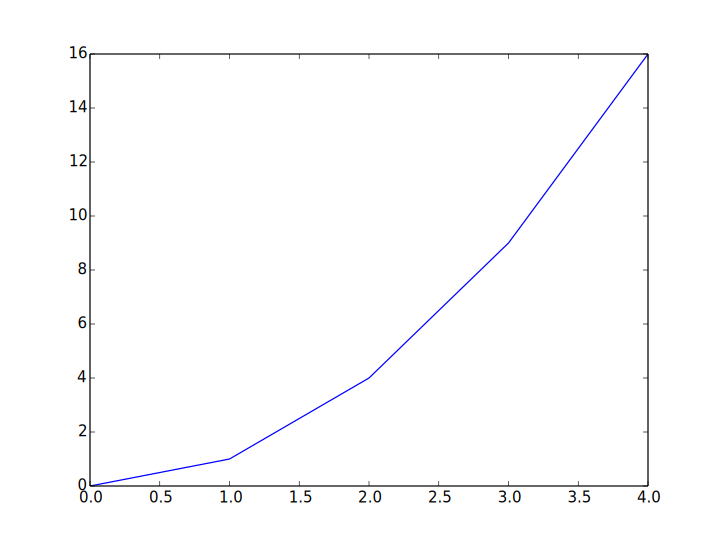
\includegraphics[width=0.6\textwidth,height=\textheight]{SciPyFigures/plot_1.*}
\caption{}
\end{figure}

\begin{figure}
\centering
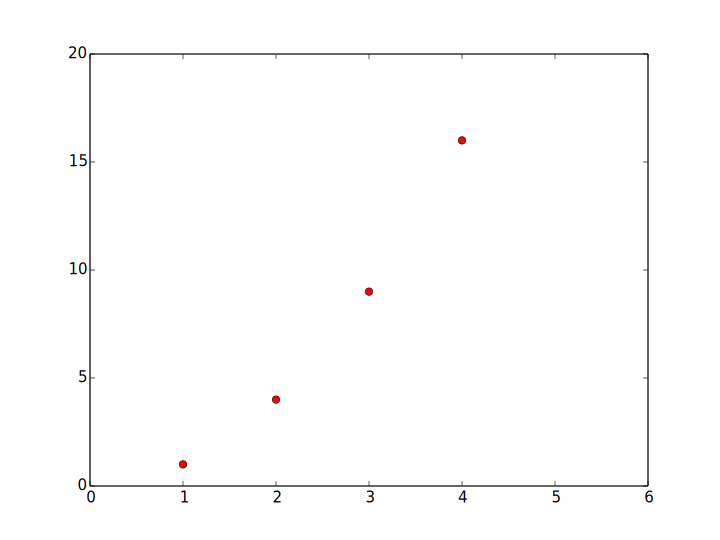
\includegraphics[width=0.6\textwidth,height=\textheight]{SciPyFigures/plot_2.*}
\caption{}
\end{figure}

This is efficiently done using NumPy arrays instead of lists and using
NumPy functions to generate the arrays.

\begin{verbatim}
In [1]: x = np.arange(0,10,0.1)

In [2]: y = np.sin(x)

In [3]: plt.plot(x,y,'b-')
Out[3]: [<matplotlib.lines.Line2D at 0x104880490>]

In [4]: plt.show()

In [5]: z = np.cos(x)

In [6]: plt.plot(y,z)
Out[6]: [<matplotlib.lines.Line2D at 0x105ea7810>]

In [7]: plt.show()
\end{verbatim}

\begin{figure}
\centering
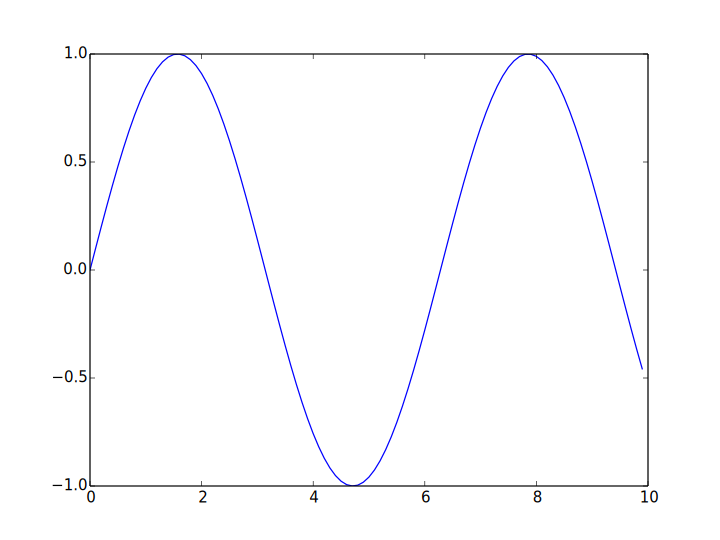
\includegraphics[width=0.6\textwidth,height=\textheight]{SciPyFigures/plot_3.*}
\caption{}
\end{figure}

\begin{figure}
\centering
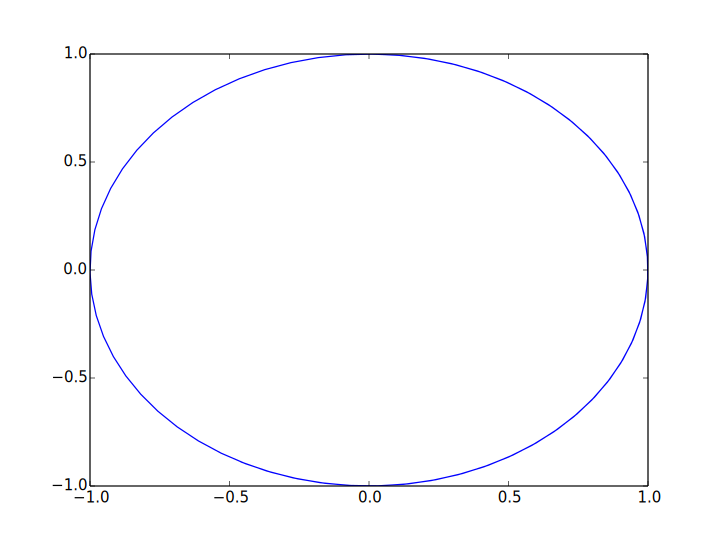
\includegraphics[width=0.6\textwidth,height=\textheight]{SciPyFigures/plot_4.*}
\caption{}
\end{figure}

Surface plots may be done by importing the library
mpl\_toolkits.mplot3d. For surface plotting to work, a meshgrid needs to
be created. This can be easily built from the x and y array data. The 3D
plotting support is in a toolit shipped wiht matplotlib. It is accessed
via the axis setting in the figure function:

\begin{verbatim}
import matplotlib.pyplot as plt
from mpl_toolkits.mplot3d import Axes3D
fig = plt.figure()
ax = fig.add_subplot(111, projection='3d')
\end{verbatim}

An example of a quadratic surface~in \texttt{plot:basicsurfaceplot}.
Many other plot examples can be found at the MatPlotLib website.

\begin{verbatim}
from mpl_toolkits.mplot3d import Axes3D
import matplotlib.pyplot as plt
import numpy as np
x = np.arange(0, 10, 0.2)
y = np.arange(0, 10, 0.2)
N,M = x.size, y.size

x,y = np.meshgrid(x,y)
z = (x-5)*(x-5) + (y-6)*(y-6)

fig = plt.figure()
ax = fig.add_subplot(111, projection='3d')
ax.plot_surface(x, y, z, rstride=1, cstride=1, color='b')
plt.show()
\end{verbatim}

Another example will illustrate both the plotting capability as well as
linear regression~\texttt{plot:fitcurveexample}.

\begin{verbatim}
import numpy as np
import matplotlib.pyplot as plt
from scipy import linalg

xl = [  0.        ,   1.11111111,   2.22222222,   3.33333333,
      4.44444444,   5.55555556,   6.66666667,   7.77777778,
      8.88888889,  10.        ]
yl = [  1.86113482,   3.81083902,   4.1465256 ,   7.37843476,
      10.76437019,  11.99975421,  14.59486508,  16.0576472 ,
      20.77206089,  20.4204027 ]

N = len(xl)
x = np.array(xl)
y = np.array(yl)
A = np.array([x, np.ones((N))]).T
AT = np.array([x, np.ones((N))])
AA = np.dot(AT,A)
ATy = np.dot(AT,y)

c = linalg.solve(AA,ATy)
t = np.arange(0,10, 0.25)
B = np.array([t,np.ones(len(t))]).T
s = np.dot(B,c)

plt.plot(t,s, 'b-', x,y, 'ro')
plt.xlim(0,10)
plt.ylim(0,20)
plt.show()






Surface plot example.







Line fit and plot example.
\end{verbatim}

\hypertarget{animation}{%
\subsubsection{Animation}\label{animation}}

Animation is done using the draw command. Create a plot with the plot
command and then update the lists using the set\_ydata command. The draw
commend will draw the updated data into the existing plot window.

\begin{verbatim}
from pylab import *
import time

ion()

tstart = time.time()               # for profiling
x = arange(0,2*pi,0.01)            # x-array
line, = plot(x,sin(x))
for i in arange(1,200):
    line.set_ydata(sin(x+i/10.0))  # update the data
    draw()                         # redraw the canvas

print 'FPS:' , 200/(time.time()-tstart)
\end{verbatim}

Interactive mode needs to be toggled using ion() and an empty plot
created. Next a loop runs through the positions of the points. The setp
command updates the plot data values. Appended to the plot values (the
plot comand) is the previous points to give the effect of a traced path.
After the animation, interactive mode is toggled, ioff() and the show()
command is executed to hold the image.

\begin{verbatim}
import numpy as np
import matplotlib.pyplot as plt
import time
from math import *

plt.ion()

line = plt.plot([],[],'ro')
plt.xlim(0, 10)
plt.ylim(0, 10)
plt.xlabel('x')
plt.ylabel('y')
plt.draw()
dt = 0.1

for t in np.arange(0,8,dt):
    x = t
    y =  x*(8-x)/2.0
    plt.setp(line,xdata = x, ydata = y)
    plt.draw()
    plt.plot([x],[y],'b.')

plt.ioff()
plt.show()
\end{verbatim}

\begin{figure}
\centering
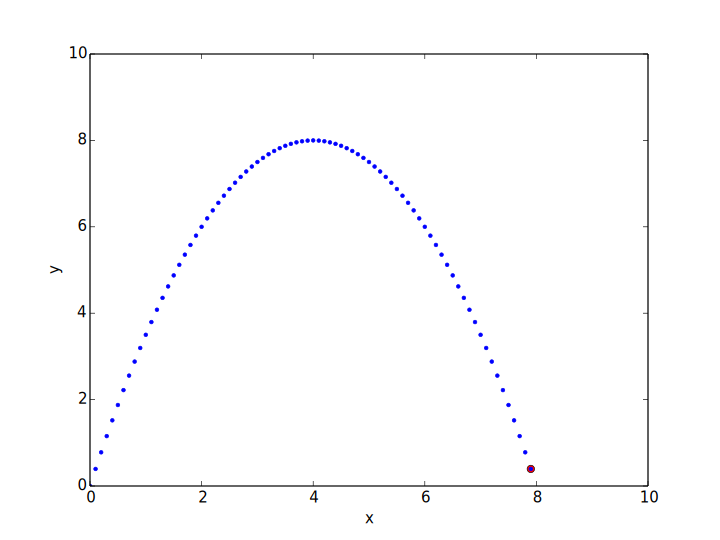
\includegraphics[width=0.6\textwidth,height=\textheight]{SciPyFigures/plot_8.*}
\caption{}
\end{figure}

Another animation example is to give virtual velocity commands to move a
point. Say you wanted to animate an object which was moving by

\[\begin{aligned}
\displaystyle \left(\frac{dx}{dt}, \frac{dy}{dt}\right) =
\left\{
\begin{array}{ll}
(0.5, 0.0),  & 0 \leq t < 2, \\[3mm]
(0.25, 1.0),  & 2 \leq t < 5, \\[3mm]
(1.0, 0.0),  & 5 \leq t < 8, \\[3mm]
(0.3, -1.0), & 8 \leq t < 10,
\end{array}
\right.
\end{aligned}\]

and starting at \(t=0\), \((x,y)  = (0.1, 3)\). Using the approximation
of the derivative

\[\displaystyle \frac{dx}{dt} \approx \frac{x(t+\Delta t) - x(t)}{\Delta t}
\quad\quad \Rightarrow \quad\quad
 \left[ x_\text{current} + \left(\frac{dx}{dt}\right) \Delta t \right] \rightarrow   x_\text{new}\]

\begin{verbatim}
import numpy as np
import matplotlib.pyplot as plt
import time
from math import *

plt.ion()

line, = plt.plot([],[],'bo')
plt.xlim(0, 10)
plt.ylim(0, 10)
plt.xlabel('x')
plt.ylabel('y')
plt.draw()
x = 0.1
y = 3
dt = 0.1


for t in np.arange(0,10,dt):
    if t < 2:
        x = x + 0.5*dt
    if (t>=2) and (t<5):
        x = x + 0.25*dt
        y = y + dt
    if (t>=5) and (t<8):
        x = x + dt
    if (t>=8):
        x = x+0.3*dt
        y = y - dt
    line.set_xdata([x])
    line.set_ydata([y])
    plt.draw()
    time.sleep(0.1)

plt.ioff()
plt.show()
\end{verbatim}

Thanks to the NumPy and SciPy online tutorials for great examples.

\hypertarget{graphing-parametric-functions}{%
\subsection{Graphing parametric
functions}\label{graphing-parametric-functions}}

The Python plot command (well, this is actually the MatPlotLib library
for Python) takes an array of x values and an array of y values. This
means that it is very easy to generate explicit plots, \(y=f(x)\) or
parametric plots, \(x=f(t)\), \(y=g(t)\). So, for example one can easily
plot a regular function via

\begin{verbatim}
import numpy as np
import pylab as plt

x = np.linspace(0,5,25) # 25 equally spaced points on [0,5]
y = 0.15*x*x*x  #  Generate the y values from y = 0.15x^3

plt.plot(x,y,'bo')  #  Plot x-y values using blue dots
plt.show()

plt.plot(x,y,'b-')  #  Plot x-y values using a blue line
plt.show()
\end{verbatim}

The two plots should look like \texttt{Fig:exampleplots}. You will
notice that the line plot hides the fact that the underlying data is
actually discrete. The point plot provides the actual points. The same
thing can be done using a parametric version making the small change in
the code:

\begin{verbatim}
t = np.linspace(0,5,25)
x = t
y = 0.15*t*t*t
\end{verbatim}

You will also notice that the space between the points is not the same
even though x (or t) was generated using uniform spacing. The x spacing
is uniform, but the y value is s nonlinear function of x and the spacing
between is not constant.

\hypertarget{code-sample-heart}{%
\subsubsection{Code Sample (heart):}\label{code-sample-heart}}

\begin{verbatim}
import numpy as np
import pylab as plt
import math
t = np.linspace(-math.pi,math.pi,200)
x = 16*(np.sin(t))**3
y = 13*np.cos(t) - 5*np.cos(2*t) - 2*np.cos(3*t) - np.cos(4*t)
plt.plot(x,y,'r-')
plt.show()
\end{verbatim}

\hypertarget{cubicsplineexample}{%
\subsubsection{Error Ellipses}\label{cubicsplineexample}}

In the section on Kalman filters, we will want to track the progress of
the filter by tracking the error of the estimate. It is normally
represented by an error ellipse where the ellipse size is the variances
or standard deviations of the Kalman estimate. Thus the larger the
standard deviations then the larger the ellipse. As you will see later
Kalman process produces a covariance, \(P\). The eigenvalues and
eigenvectors of \(P\) can be used for the basic variance information.
The eigenvectors represent the major and minor axis directions and the
eigenvalues represent the lengths of those axes. Note: in some
applications it makes sense to graph the standard deviations instead of
the variances and so one should take the square root of the eigenvalues.
The algorithm follows.

\begin{itemize}
\tightlist
\item
  Compute the eigenvalues and eigenvectors of \(P\):
  \((\lambda_1, v_1)\), \((\lambda_2, v_2)\). Call the larger one \(a\)
  and the smaller one \(b\).
\item
  Compute the square roots of the eigenvalues IF desired (if the
  variances are really small or really huge).
\item
  Compute the smaller angle between the eigenvector and the \(x\)-axis.
  Call this \(\theta\) and assume it is for \(v_1\).
\item
  Call an ellipse routine to plot.
\end{itemize}

Let a, b be the major and minor axis lengths, x0, y0 be the center and
angle be the tilt angle. The function to plot an rotated ellipse is
given by:

\begin{verbatim}
def Ellipse(a,b,angle,x0,y0):
    points=100
    cos_a,sin_a=math.cos(angle*math.pi/180),math.sin(angle*math.pi/180)
    theta=np.linspace(0,2*np.pi,points)
    X=a*np.cos(theta)*cos_a-sin_a*b*np.sin(theta)+x0
    Y=a*np.cos(theta)*sin_a+cos_a*b*np.sin(theta)+y0
    return X,Y
\end{verbatim}

The following is an example of how to plot an error ellipse for the
covariance matrix

\[\begin{aligned}
P = \begin{pmatrix} 0.9 & 0.1 \\ 0.1 & 0.5 \end{pmatrix}
\end{aligned}\]

about the point \((4,5)\). We use the eigenvalues and eigenvectors to
plot the major and minor axes. The following is a quick example on how
to extract eigenvalues and plot an ellipse.

\begin{verbatim}
import math
import numpy as np
import pylab as plt
from numpy import linalg
P = np.array([[0.9, 0.1],[0.1, 0.5]])
w, v = linalg.eig(P)
angle = 180*math.atan2(v[1][0],v[0][0])/math.pi
u,v = Ellipse(w[0],w[1],angle, 4,5)
fig = plt.figure()
ax = fig.add_subplot(111)
ax.plot(u,v,'b-')
ax.set_aspect('equal')
fig.savefig("Ellipse.pdf")
plt.show()
\end{verbatim}

\begin{figure}
\centering
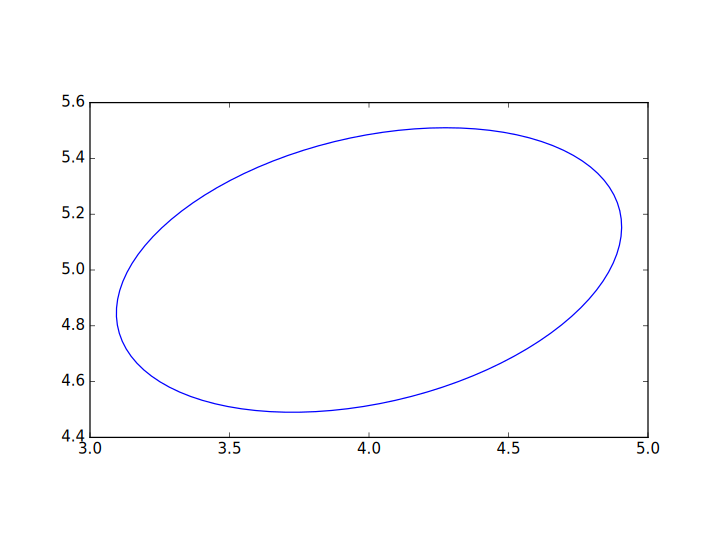
\includegraphics[width=0.7\textwidth,height=\textheight]{SciPyFigures/Ellipse.*}
\caption{Tilted ellipse}
\end{figure}

\hypertarget{data-plots}{%
\subsubsection{Data Plots}\label{data-plots}}

To plot the data used in the curve fitting examples:

\begin{verbatim}
import numpy as np
import pylab as plt
x = []
y = []
f = open('data.txt','r')
for line in f:
  item = line.split()
  xt = eval(item[0])
  yt = eval(item[1])
  x.append(xt)
  y.append(yt)

plt.plot(x,y, 'ro')
plt.show()
\end{verbatim}

For Figure in subsection \texttt{plot:quadgraph}:

\begin{verbatim}
import numpy as np
import pylab as plt
from scipy import linalg

xl = []
yl = []
f = open('data.txt','r')
for line in f:
  item = line.split()
  xt = eval(item[0])
  yt = eval(item[1])
  xl.append(xt)
  yl.append(yt)

N = len(xl)
x = np.array(xl)
y = np.array(yl)
xx = x*x
A = np.array([xx, x, np.ones((N))]).T
AT = np.array([xx, x, np.ones((N))])
AA = np.dot(AT,A)
ATy = np.dot(AT,y)

c = linalg.solve(AA,ATy)
t = np.arange(0,3, 0.1)
tt = t*t
B = np.array([tt,t,np.ones(len(t))]).T
s = np.dot(B,c)

plt.plot(t,s, 'b-', x,y, 'ro')
plt.xlim(0,3)
plt.ylim(0,2)
plt.show()
\end{verbatim}

Note that NumPy/SciPy provides some built in functions to fit
polynomials to lines. The NumPy function linalg.lstsq will compute the
pseudoinverse via the normal equations directly and the NumPy function
polyfit will do this assuming you are fitting a polynomial. In terms of
speed, doing it ourselves tends to be fastest, with the next fastest is
the lstsq function and the polyfit function the slowest.

\textbf{Footnotes}
